\documentclass{exam}
\usepackage{../../scripts/commonheader}
\usepackage{enumitem}
\usepackage{changepage}
\usepackage{amsmath,amssymb,amsthm}
\usepackage[thinlines]{easytable}
\usepackage{tabu}
\usepackage{array}
\newcolumntype{C}[1]{>{\centering\let\newline\\\arraybackslash\hspace{0pt}}m{#1}}
\usepackage{tabulary}
%to insert images
\usepackage{graphicx}
% to use :=
\usepackage{mathtools} 
\usepackage{wrapfig}
\usepackage[table]{colortbl}% http://ctan.org/pkg/xcolor
\graphicspath{ {../images/} }

\renewcommand{\HRule}[1][\medskipamount]{\par
  %\vspace*{\dimexpr-\parskip-\baselineskip+#1}
  \noindent\rule{\linewidth}{0.2mm}\par}
   \renewcommand\tab[1][1cm]{\hspace*{#1}}
\renewcommand{\qedsymbol}{\rule{0.7em}{0.7em}}
\newcolumntype{L}{>{\centering\arraybackslash}m{3cm}}
%%% Change these %%%%%%%%%%%%%%%%%%%%%%%%%%%%%%%%%%%%%%%%%%%%%%%%%%%%%%%%%%%%%%

\discnumber{1}
\title{\textsc{Mentor Guide to LLSE}}
\date{November 14 to November 18, 2016}

%%%%%%%%%%%%%%%%%%%%%%%%%%%%%%%%%%%%%%%%%%%%%%%%%%%%%%%%%%%%%%%%%%%%%%%%%%%%%%%

\begin{document}


\maketitle
\rule{\textwidth}{0.15em}
\fontsize{12}{15}\selectfont
\thispagestyle{empty}

\section{Covariance}
\subsection{Formulas}
Provided that $X$ and $Y$ are random variables, we define \textbf{covariance} as follows:
\[\cov(X, Y) = \E((X - \E(X)) \cdot (Y - \E(Y)))\]

\textbf{Claim:} $\cov(X, Y) = \E(XY) - \E(X)\E(Y)$
\begin{align*}
\E((X - \E(X)) \cdot (Y - \E(Y))) \\
&= \E(XY - \E(X)Y - X\E(Y) + \E(X)\E(Y))\\
&= \E(XY) - \E(X)\E(Y) - \E(X)\E(Y) + \E(X)\E(Y)\\
\intertext{We can cancel out the last two terms:}
&= \E(XY) - \E(X)\E(Y)
\end{align*}

\subsection{Intuition}
Look at the following graphs. What is the covariance of each? If $X$ increases, what happens to $Y$? Are these events independent? Does uncorrelated imply independence? Does independence imply uncorrelated?

\begin{minipage}[b]{0.3\linewidth}
\begin{center}
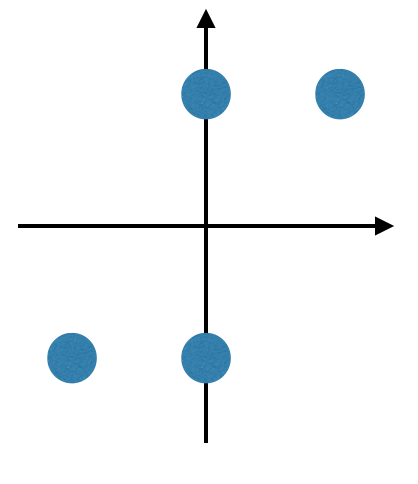
\includegraphics[width=2cm]{llse_cov2.jpg}
\end{center}
\end{minipage}%
\hfill
\begin{minipage}[b]{0.3\linewidth}
\begin{center}
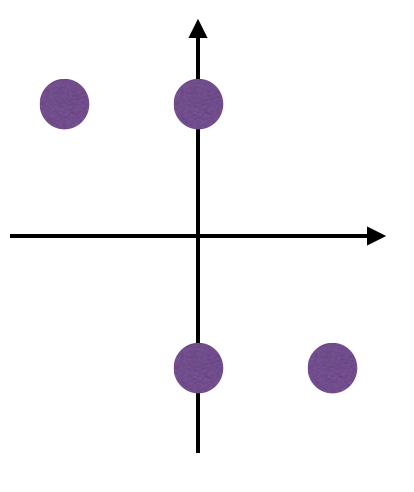
\includegraphics[width=2cm]{llse_cov1.jpg}
\end{center}
\end{minipage}%
\hfill
\begin{minipage}[b]{0.3\linewidth}
\begin{center}
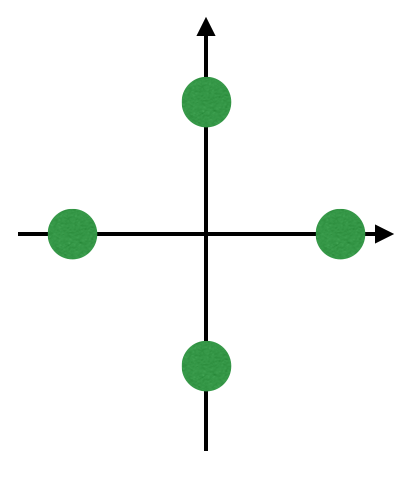
\includegraphics[width=2cm]{llse_cov3.jpg}
\end{center}

\end{minipage}

\subsection{Properties of Covariance}
\begin{enumerate}
\item $\var(X)  = \cov(X, X)$
\item $X$, $Y$ independent $\rightarrow$ $\cov(X, Y) = 0$. Independent random variables are uncorrelated. The converse is not necessarily true (look at the last example on the previous page).
\item $\cov(a + X, b + Y) = \cov(X, Y)$
\item $\cov(aX + bY, cU + dV) = ac \cdot \cov(X, U) + ad \cdot \cov(X, V) + bc \cdot \cov(Y, U) + bd \cdot \cov(Y, V)$
\end{enumerate}

\textbf{Proofs}
\begin{enumerate}
\item Plug into original equation.
\item Plug into original equation (see what you can cancel out by applying the definition of covariance and independence of the variables).
\item Plug into original equation. 
\item This one is a little tricky. Since we know that we can add and subtract \textbf{constants}, we can zero mean the variables. So we can assume that $\E(aX + bY) = \E(cU + dV) = 0$. Now let's apply the definition of covariance.
\begin{align*}
\cov(aX + bY, cU + dV) \\
\intertext{ Since $\E(aX + bY) = \E(cU + dV) = 0$, we get}
&= \E((aX + bY) \cdot (cU + dV)) - 0 \cdot 0 \\
\intertext{By linearity of expectation:}
&= ac \cdot \E(XU) + ad \cdot \E(XV)  + bc \cdot \E(YU) + bd \cdot \E(YV) \\
\intertext{Now note that $\cov(X, U) = \E(XU) - \E(X)\E(U) = \E(XU) - 0\cdot 0 = \E(XU)$}
\intertext{Apply the above result to each term to get:}
&= ac \cdot \cov(XU) + ad \cdot \cov(XV)  + bc \cdot \cov(YU) + bd \cdot \cov(YV)
\end{align*}
\end{enumerate}

\clearpage 

\section{LLSE}
\subsection{Constant}
\textbf{Motivation: } Say we have a random variable $Y$, which measures height. What would be our best guess for $Y$? In other words, if a random person called us, what would be our best guess for their height?

\subsection{Minimizing Error}
We need to first somehow quantify "the best guess".  When we choose a number for height, how do we know that the number we chose is a good gues? It makes sense to pick such a number, where the error is minimized. We will look at the \textbf{mean square error},
\[\E((Y - a)^2)\]
and show that this equation achieves a minimum value only when $a = \E(Y)$.

Define 
\[\hat{Y} = Y - \E(Y)\]
$\hat{Y}$ is the error we make by using $\E(Y)$ to estimate $Y$.

Note that,
\[\E(\hat{Y}) = \E(Y - \E(Y)) = \E(Y) - \E(\E(Y)) = \E(Y) - \E(Y) = 0\]

This implies that $\E(\hat{Y}\cdot c) = 0  \forall c$

Now we will use these facts to show that if $a$ is any constant other than $\E(Y)$, the mean square error will be larger than if we had used $\E(Y)$.

\begin{align*}
\E((Y - a^2)) &= \E((Y - \E(Y) + \E(Y) - a)^2) && \text{trick}\\
&= \E((\hat{Y} + c)^2) && \text{where $c = \E(Y) - a$}\\
&= \E(\hat{Y}^2 + 2\hat{Y}c + c^2) && \text{expand the square}\\
&= \E(\hat{Y})^2 + 2\E(\hat{Y}c) + c^2 && \text{linearity of expectation}\\
&= \E(\hat{Y})^2 + 0 + c^2 && \text{using fact from above}\\
&\geq \E(\hat{Y}^2) && \text{$c^2 \geq 0$}
\end{align*}
Hence, 
\[\E((Y - a)^2) \geq \E((Y - \E(Y))^2)\]

\clearpage

\subsection{Linear}
We now have a good estimate for $Y$ if we have no additional information. However, what if we know some samples of $Y$ and some other random variable $X$. For example, say we know the weight of the caller. We should be better able to guess their height, as there is some sort of correlation between weight and height. However, the model we are using so far does not apply any additional information to the guess.  Let us construct a new way to predict $Y$, based on some observed $X$.

Continuing the example we have been using so far with height and weight, assume we are given the the points shown below. 

\begin{center}
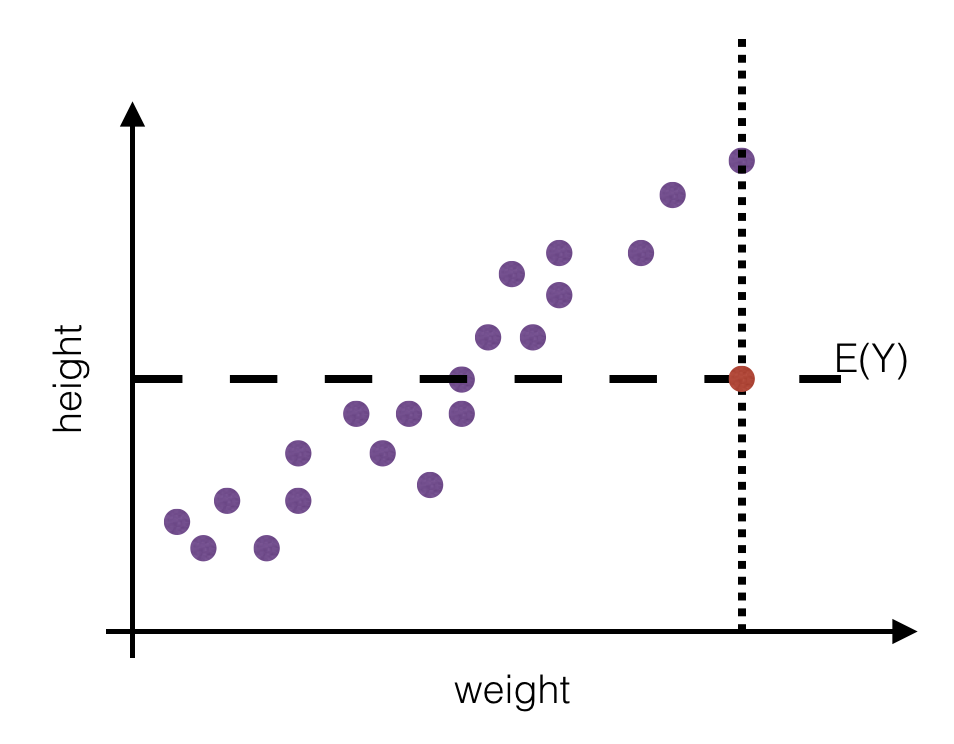
\includegraphics[width=8cm]{llse_linear.jpg}
\end{center}

We can see that $\E(Y)$ is not a good guess given additional information. We wish to construct a linear equation which given a value of $X$, will predict the value of $Y$. So if someone calls you and provides their weight, you can more accurately predict what their height is.

So far, our example has been non Bayesian, meaning we did not know the distributions of $X$ and $Y$. We will develop the linear least square estimate using $X$, $Y$ with known distributions. Then we will see how we can apply these results to non Bayesian stuff.

\textbf{Theorem}
Assume $X$, $Y$ are random variables with known distribution. Then, 
\[\L[Y | X] = \E(Y) + \frac{\cov(X, Y)}{\var(X)} \cdot (X - \E(X)) = \hat{Y}\]

We want to show that the mean square between $Y$ and $\hat{Y}$ is smaller than between $Y$ and any other linear function of $X$. We will use a technique similar to how we showed the constant case.

\clearpage

\subsection{First Proof of $L[Y | X]$}
Recall,
\[\hat{Y} = \E(Y) + \frac{\cov(X, Y)}{\var(X)} \cdot (X - \E(X))  \]
Plug the above equation into the mean value of the error:
\begin{align*}
Y - \hat{Y} &= Y - \E(Y) - \frac{\cov(X, Y)}{\var(X)} \cdot (X - \E(X))\\
\E(Y - \hat{Y}) &= \E\bigg(Y - \E(Y) - \frac{\cov(X, Y)}{\var(X)} \cdot (X - \E(X))\bigg)\\
&= \E(Y - \E(Y)) - \frac{\cov(X, Y)}{\var(X)} \E(X - \E(X))\\
&= 0 - 0 = 0
\end{align*}
So we know that the mean value of the error is 0.

\textbf{Claim: } $\E((Y - \hat{Y})X) = 0$

\textbf{Proof of claim:}

Note,
\[\E((Y - \hat{Y})X) = \E((Y - \hat{Y}) \cdot (X - \E(X)))\]
To see that the two sides are equivalent we do the following:  expand the LHS and apply linearity of expectation we get,
\begin{align*}
\E((Y - \hat{Y}) \cdot (X - \E(X))) &= \E(YX - \hat{Y}X - Y \E(X) + \hat{Y} \E(X))\\
&= \E(YX - \hat{Y}X) - \E(X) \E(Y - \hat{Y}) && \text{mean value of error is 0}\\
&= \E(YX - \hat{Y}X) = \E((Y - \hat{Y})X)
\end{align*}

Now simplify the new equation, $\E((Y - \hat{Y}) \cdot (X - \E(X)))$:
\begin{align*}
\E((Y - \hat{Y}) \cdot (X - \E(X))) &= \E \Bigg( \bigg(Y - \bigg(\E(Y) + \frac{\cov(X, Y)}{\var(X)} \cdot (X - \E(X))\bigg) \cdot (X - \E(X)) \Bigg)\\
&= \E((Y - \E(Y))(X - \E(X))) - \frac{\cov(X, Y)}{\var(X)} \E((X - \E(X))(X - \E(X)))\\
&= \cov(X, Y) - \frac{\cov(X, Y)}{\var(X)} \var(X) \\
&= 0
\end{align*}

We conclude that $\E((Y - \hat{Y})X) = 0$.

\clearpage

We need one more fact in order to prove our original claim:

\textbf{Claim: } The error is orthogonal to all linear functions. (We have shown that it is orthogonal to $x$)

\textbf{Proof of claim:} 
\begin{align*}
\E((Y - \hat{Y}) (c + dX)) &= \E(Yc - \hat{Y}c + YdX - \hat{Y}dX)\\
&= c\E(Y - \hat{Y}) + d\E((Y - \hat{Y})X)\\
&= 0 - 0 = 0 && \text{using above results}
\end{align*}


Now let's get back to our original claim: We want to show that the mean square between $\hat{Y}$ and $Y$ is smaller than between $Y$ and any other linear function. Recall that to show $\E(Y)$ is the best constant estimate for $Y$ we proved the following equation: 
\[\E((Y - a)^2) \geq \E((Y - \E(Y))^2)\]

To show that $\hat{Y}$ is the best linear estimator for $Y$, we will prove that 
\[\E((Y - a - bX)^2) \geq \E((Y - \hat{Y})^2)\]

Note the following relation:
\[\E((Y - \hat{Y})(\hat{Y} - a - bX))  = 0 \forall a, b\]

We have shown that error is orthogonal to all linear functions. $\hat{Y}$ and $-a - bX$ are both linear functions, so adding them produces a linear function.

Now we use this fact to prove the inequality:

\begin{align*}
\E((Y - a - bX)^2) &= \E((Y - \hat{Y} + \hat{Y} - a - bX)^2)\\
&= \E((Y - \hat{Y})^2) + \E((\hat{Y} - a - bX)^2) + 0\\
&\geq \E((Y - \hat{Y})^2) && \text{as $\E((\hat{Y} - a - bX)^2) \geq 0$}
\end{align*}

We have shown that the mean square error from using $a + bX$ is always going to be larger than if we used $\hat{Y}$.

\clearpage

The diagram below offers a visualization of the above facts (from Walrand)
\begin{center}
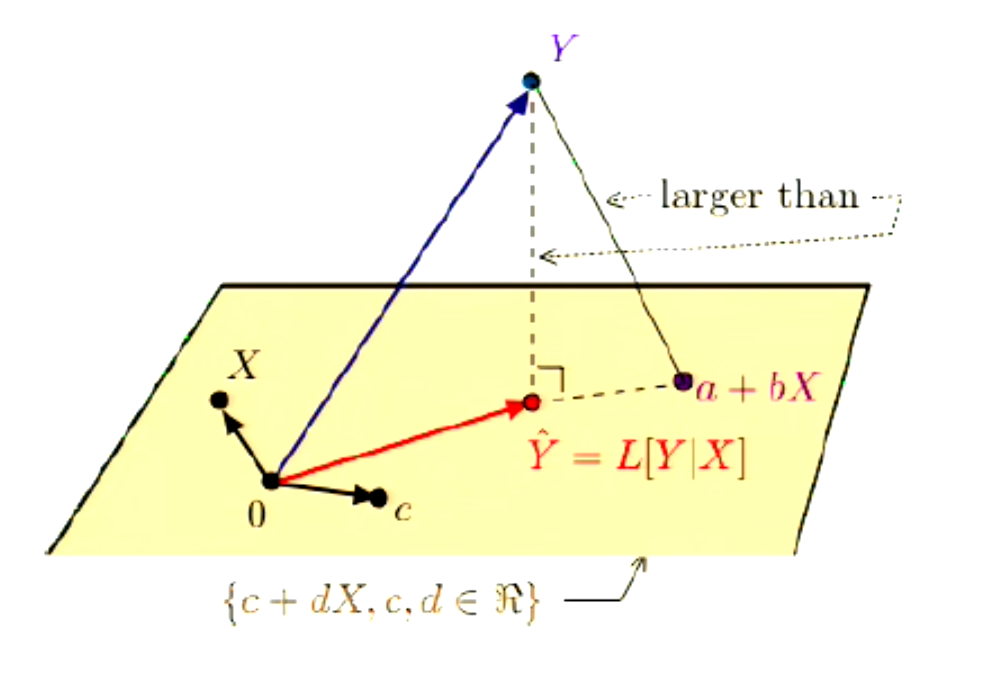
\includegraphics[width=5cm]{llse_projection.jpg}
\end{center}
It also demonstrates the \textbf{Projection Property}. If the plane is the set of all linear functions of X, then $Y - \hat{Y}$ is orthogonal (perpendicular) to any linear function of X (or the plane).

Here is another derivation of  $\hat{Y}$ using a calculus approach.

\subsection{Second Proof of $L[Y | X]$}

Assume that $\E(X) = \E(Y)  = 0$.  
\[\hat{Y} = \E(Y) + \frac{\cov(X, Y)}{\var(X)} \cdot (X - \E(X)) =   \frac{\cov(X, Y)}{\var(X)} \cdot X\]
We want to find $a$ and $b$ such that $g(a, b)$ is minimized, where $\hat{Y} = a + bX$
\begin{align*}
g(a, b) &= \E((Y - a - bX)^2)\\
&= \E(Y^2 + a^2 + b^2 X^2 - 2aX - 2bXY + 2bX)\\
&= a^2 + \E(Y^2) + b^2\E(X^2) - 2a\E(Y) - 2b\E(XY) + 2b\E(X)\\
&= a^2 + \E(Y^2) + b^2\E(X^2) - 2b\E(XY) && \text{X, Y are zero mean}
\end{align*}

To find the minimum value of $g(a, b)$ take the partial derivatives with respect to $a$ and $b$ and set them both to zero. Then solve to find $a$ and $b$.
\begin{align*}
0 &= \frac{\partial }{\partial a} g(a, b) = 2a \rightarrow a = 0\\
0 &= \frac{\partial }{\partial b} g(a, b) = 2b \E(X^2) - 2\E(XY) \rightarrow b = \frac{\E(XY)}{\E(X^2)} = \frac{\cov(X, Y)}{\var(X)}
\end{align*}
The last line follows from the fact that $X$ and $Y$ are zero mean:
\begin{align*}
\cov(X, Y) &= \E(XY) - \E(X)\E(Y) = \E(XY) - 0 \cdot 0 = \E(XY)\\
\var(X) &= \E(X^2) - \E(X)^2 = \E(X^2) - 0 = \E(X^2)
\end{align*}
\[\hat{Y} = a + bX = 0 + \frac{\cov(X, Y)}{\var(X)} \cdot X \]
This proves that $\hat{Y}$ is the best linear estimate for $Y$.



In the above proof we forced $X$ and $Y$ to be zero mean. We can use a similar proof technique with any $X$ and $Y$.

\subsection{Third Proof of $L[Y | X]$}
This applies the second proof to $X$ and $Y$ that are not zero mean. This proof is not covered in lecture and basically involves maneuvering terms around, so read it if you're curious.
\begin{align*}
Y - a - bX &= Y - \E(Y) - (a - \E(Y)) - b(X - \E(X)) - b \E(X) && \text{add some magic terms}\\
&= Y - \E(Y) - (a - \E(Y) + b \E(X)) - b(X - \E(X)) && \text{rearrange terms}\\
&= Y - \E(Y) - c - b(X - \E(X)) && \text{$c = a - \E(Y) + b \E(X)$}
\end{align*}
Now apply results from the Second Proof of $L[Y | X]$, since $Y - \E(Y) $ and $X - \E(X)$ are both zero mean. 
\begin{align*}
c & = 0 \rightarrow 0 = a - \E(Y) + b \E(X) \rightarrow a = \E(Y) - b\E(X)\\
b &= \frac{\cov(X - \E(X), Y - \E(Y))}{\var(X - \E(X))} = \frac{\cov(X, Y)}{\var(X)}
\end{align*}

Now plug in the above results into $a + bX$:
\begin{align*}
a + bX &= \E(Y) - b\E(X) + bX\\
&= \E(Y) - b (-\E(X) + x) = \E(Y) + \frac{\cov(X, Y)}{\var(X)}(X - \E(X))
\end{align*}

\subsection{Some General Comments about LLSE}
\[\L[Y | X] = \E(Y) + \frac{\cov(X, Y)}{\var(X)} \cdot (X - \E(X))\]
\begin{enumerate}
\item Covariance controls the slope of LLSE (variance is always positive). If the covariance is positive, then as $X$ increases, our prediction for $Y$ will also increase.
\item If you know the distributions of $X$ and $Y$, you can calculate each component of the above equation.
\item If $X$ and $Y$ are independent, then the best guess is $\E(Y)$
\item If we have no observations, the best choice for an estimate of $Y$ is $\E(Y)$. In this case, the mean error would be:
\[\E((Y - \E(Y))^2) = \var(Y)\]
\item Observing $X$ will reduce the error. The error depends on how $X$ and $Y$ are correlated and is defined as follows:
\[\E((Y - \L[Y | X] = \var(Y) - \frac{\cov(X, Y)^2}{\var(X)}\]
Note that both the numerator and denominator in the fraction are nonnegative. Since the error of using $\E(Y)$ is $\var(Y)$, the error of using $\L[Y | X]$ will always be smaller than if we just used $\E(Y)$. 
\end{enumerate}

\subsection{Bayesian and non Bayesian}
We motivated this section with a non Bayesian example. Then we used Bayesian stuff in all of our proofs. Now we explain that Bayesian and non Bayesian are really the same thing.

\textbf{non Bayesian}

Given samples: $\{\(X_n, Y_n\) n = 1,  \dotsc N \}$
We want 
\[\hat{Y} = a + bX\]
where $a$, $b$ minimize
\[\sum_{n = 1}^{N} (Y_n - a - bX_n)^2\]

In other words, we minimize the square of the distance between the line and the points. We take the square of the distance because taking the absolute value of the difference is more complicated.

Note that in the above formulation, we made no assumptions about the distribution of $X$.

\textbf{Bayesian}

Given $X$, $Y$ with known distribution. We want:
\[\hat{Y} = a + bX = \L[Y | X]\]
where
\[g(a, b) = \E((Y - a - bX)^2)\]
is minimized.

We can turn non Bayesian into Bayesian as follows:

\[\frac{1}{N} \sum (Y_n - a - bX_n)^2 = \E((Y - a - bX)^2)\]
\[(X, Y) = (X_n, Y_n) \text{ w. p. } \frac{1}{N} \text{ for } n = 1, \dotsc, N\]

\clearpage

\section{Example of Finding LLSE  (non Bayesian)}
Find the linear least square estimate of the following joint distribution.
\begin{center}
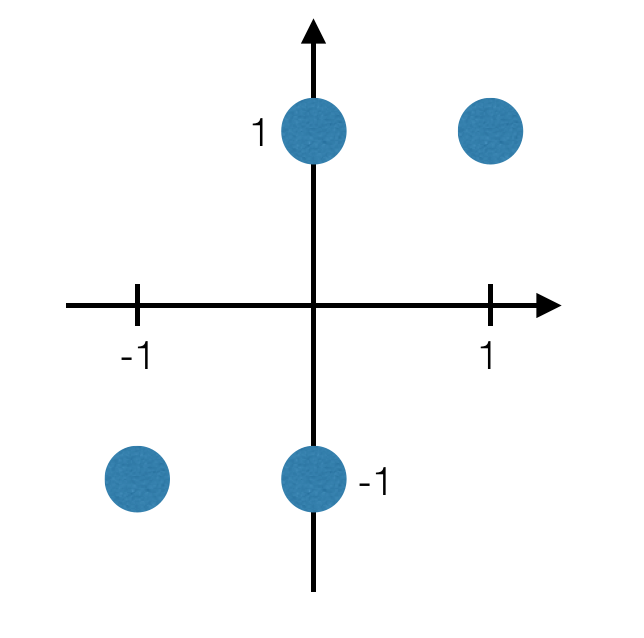
\includegraphics[width=5cm]{llse_simpleex.jpg}
\end{center}

We turn the problem from non Bayesian into Bayesian by assuming that the 4 points are equally likely values of $(X, Y)$.

\begin{align*}
\E(X) &= -1 \cdot \frac{1}{4} + 0 \cdot \frac{1}{2} + 1 \cdot \frac{1}{4}\\
\E(Y) &= -1\cdot \frac{1}{2} + 1 \cdot \frac{1}{2} = 0\\
\E(X^2) &= (-1)^2 \cdot \frac{1}{4} + (0)^2 \cdot \frac{1}{2} + (1)^2 \cdot \frac{1}{4} = \frac{1}{2}\\
\E(XY) &= 1 \cdot \frac{1}{2} = \frac{1}{2}\\
\var(X) &= \E(X^2) - \E(X)^2 = \frac{1}{2} - 0 = \frac{1}{2}\\
\cov(X, Y) &= \E(XY) - \E(X) \E(Y) = \frac{1}{2} - 0 = \frac{1}{2}
\end{align*}
Therefore we get: 
\[\L[Y | X] = 0 + \frac{\frac{1}{2}}{\frac{1}{2}} \cdot X = X\]

\clearpage

\section{Conditional Expectation}

\textbf{Motivation}

There are situations where the relationship between $X$ and $Y$ is non linear. Our goal is to find $g(\cdot)$ such that $g(X)$ is the best guess about $Y$ given $X$ where $g(\cdot)$ is not restricted to a line.

\subsection{Motivating Example}
Examine the following joint distribution of $X$ and $Y$. 
\begin{center}
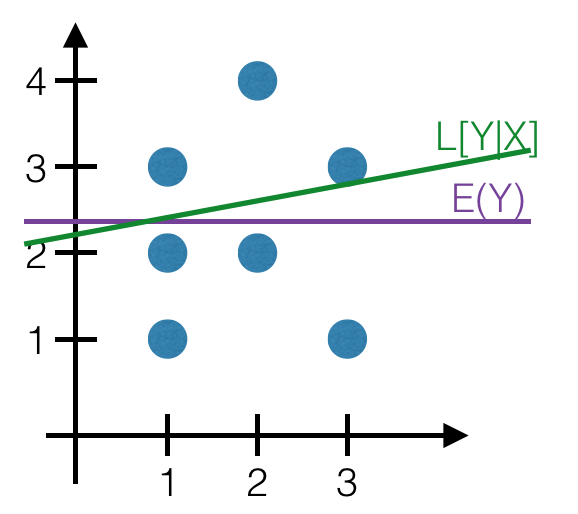
\includegraphics[width=5cm]{llse_condexp.jpg}
\end{center}

Without any observations, our best guess for $Y$ is $\E(Y) = 2.3$. Assuming we observe $X$, we can construct the following linear estimate: 
\[\L[Y | X ]  = a + bX = 2.1 + 0.1X\]

What if we know that $X$ is 1? What would be our best guess for $Y$ in that case? 2! Since there are 3 values that $Y$ can take on one we know that $X$ is 1, we find the average of those values. So once we narrow down $X$, we examine a new distribution. Repeating this process for each value of $X$ gives us the following diagram:

\begin{center}
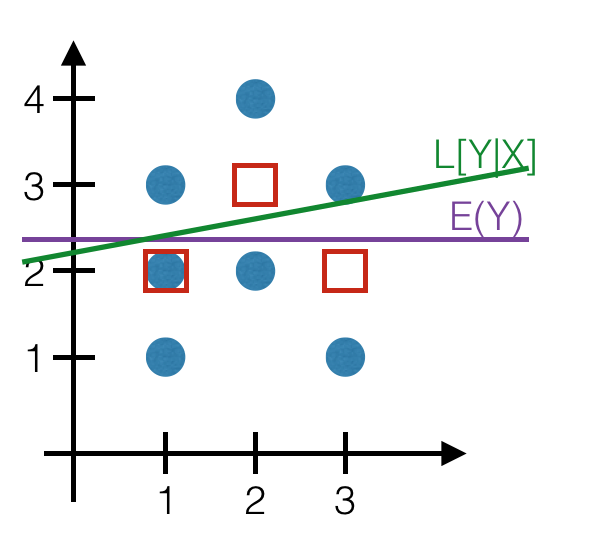
\includegraphics[width=5cm]{llse_condexp2.jpg}
\end{center}

Compare the each of the new expected values with what the linear equation gives us. Which is closer?

\clearpage

\subsection{Defining Conditional Expectation}

If $X$ and $Y$ are random variables in $\Omega$ then the \textbf{conditional expectation} is defined as follows:
\begin{align*}
\E(Y | X) &= g(X) \\
\text{ where, } g(X) &= \E(Y | X = x) \\
&= \sum_{y} y \cdot \P[Y=y | X = x] \\
&\text{with } \P[Y=y | X=x] = \frac{\P[X=x, Y=y]}{\P[X=x}
\end{align*}

\textbf{Theorem}

$\E(Y | X)$ is the best guess about $Y$ given $X$.
\[\E((Y - g(X))^2) \geq \E((Y - \E(Y | X))^2)\]
Using any other function to predict $Y$ will give a larger error.

\subsection{Projection Property Revisited}

\textbf{Projection Property: } $\E((Y - \E(Y | X))f(X)) = 0 \forall f(\cdot)$

This is equivalent to the following, 
\begin{align*}
\E((Y - \E(Y | X))f(X)) &= \E(Y \cdot f(X) )- \E(\E(Y | X) \cdot f(X))\\
&\rightarrow\\
\E(Y \cdot f(X)) &= \E(\E(Y | X) f(X))
\end{align*}

\textbf{Proof:}
\begin{align*}
\E(\E(Y | X) \cdot f(X)) &= \sum_{x} \E(Y | X = x) \cdot f(x) \cdot \P[X = x]\\
&= \sum_{x} \bigg(\sum_{y} y \cdot f(x) \cdot \P[Y = y | X = x] \bigg) \cdot \P[X = x]\\
&= \sum_x \sum_y y \cdot f(x) \P[X = x, Y = x] && \text{ using $\frac{\P[X=x, Y=y]}{\P[X=x]}$}\\
&= \E(Y \cdot f(X))
\end{align*}

Therefore, if we have the conditional expectation, we can take its mean value and get the mean value of $Y$.

\clearpage

\subsection{CE = MMSE}
Finally we prove the fact that $\E(Y | X)$ is the best guess about $Y$ based on $X$. We use a technique similar to before.

Recall, 
\begin{align*}
\E(Y | X) &= g(X) \\
\text{ where, } g(X) &= \E(Y | X = x) \\
&= \sum_{y} y \cdot \P[Y=y | X = x] \\
&\text{with } \P[Y=y | X=x] = \frac{\P[X=x, Y=y]}{\P[X=x}
\end{align*}

We want to show that $g(X)$ minimizes $\E((Y - g(X))^2)$. Let $h(X)$ be any other function.

\begin{align*}
\E((Y - h(X))^2) &= \E((Y - g(X) + g(X) - h(X))^2) && \text{add in some magic terms}\\
&= \E((Y - g(X))^2) + \E((g(X) - h(X))^2) \\
&+ 2\E((Y - g(X))(g(X)-h(X)) && \text{linearity of expectation}\\
\end{align*}

We know that $\E((Y - g(X))(g(X)-h(X)) = 0$ by the Projection Property and $\E((g(X) - h(X))^2 \geq 0$.

Therefore, 
\[\E((Y - h(X))^2) \geq \E((Y - g(X))^2)\]
\end{document}
